\documentclass[a4paper, oneside, 12pt]{article}
\usepackage{amsmath} % http://ctan.org/pkg/amsmath
\usepackage{graphicx}
\usepackage{caption}
\usepackage{subcaption}
\usepackage{scrextend}
\usepackage{listings}
\usepackage{ragged2e}
\usepackage{hyperref}
\usepackage{gensymb}
\usepackage[utf8]{inputenc}
\usepackage{tikz}
\usepackage{floatrow}
\usepackage[export]{adjustbox}
\usetikzlibrary{matrix,shapes,arrows,positioning,chains}
\usepackage[margin=1in]{geometry}
\usepackage{wrapfig}
\usepackage{listings}



%%NOTE YOU MUST HAVE  BIBTEX FILE FOR THE BILIOGRAPHY AND REFERENCING TO WORK
% I use Mendeley to automatically generate this from my library of papers
% simply type \cite{Amazon2018} to cite it within the paper, with 'Amazon2018' being the citation key in this case

%%%%%%%%%%%LATEX EXAMPLES%%%%%%%%%%%%%%


%%%%INSERT A FIGURE	
%\begin{figure}[!!h]  %%!!h ensures it is in same order in pdf as within the latex file
%	\centering
%	\begin{subfigure}{0.18\textwidth}
%		\includegraphics[width=1\textwidth]{FaceDetectOutput4.jpg}
%		\caption{Dart4.jpg}
%		\label{fig::1a}
%	\end{subfigure}
%	~
%	\begin{subfigure}{0.22\textwidth}
%		\includegraphics[width=1\textwidth]{FaceDetectOutput5.jpg}
%		\caption{Dart5.jpg}
%		\label{fig::1b}
%	\end{subfigure}	
%	\caption{Detections from the frontal face cascade, red boxes indicate a true positive detection and turquoise boxes indicate a false positive detection.}
%	\label{fig::1}
%\end{figure}

%%% TO CITE THE FIGURE \ref{fig::1}
%% YOU CAN HAVE DIFFERENT TYPES E.G. \ref{table::1}, just remember to change the label

%%%%DRAW A FLOWCHART
%\begin{tikzpicture}
%\matrix (m)[matrix of nodes, column  sep=2cm,row  sep=8mm, align=center, nodes={rectangle,draw, anchor=center} ]{
%	|[block]| {1. Recieve V-J detection frames and Hough Transform detection frames.}              &  |[block]| {8. Classify the V-J detection frame as a true detection.}            \\
%	|[block]| {2. Define Hough tolerance parameters and derive bounds based on V-J detection frame width and height.}         &           |[decision]| {7. Coordinates correspond to pre-defined bottom right corner of Hough transform detection frame.}                                   \\
%	|[block]| {3. Search around top left corner of V-J detection frame within bounds.}    &    |[block]| {6. Repeat 3. for bottom right corner of V-J detection frame.}                                           \\
%	|[decision]| {4. Top left corner of Hough transform detection frame detected}         &       |[block]| {5. Run along top of frame and then down the side to bottom left corner of Hough transform detection frame.}                                      \\
%};
%\path [line] (m-1-1) -- (m-2-1);
%\path [>=latex,->] (m-2-1) edge (m-3-1);
%\path [>=latex,->] (m-3-1) edge (m-4-1);
%%\draw[->] (m-3-1) -{Yes}- (m-4-1);
%\path [line] (m-4-1) -- node[above] {\textbf{Yes}} (m-4-2);
%\path [>=latex,->] (m-4-2) edge (m-3-2);
%\path [>=latex,->] (m-3-2) edge (m-2-2);
%\path [line] (m-2-2) -- node[left] {\textbf{Yes}} (m-1-2);
%\end{tikzpicture}


%%EQUATION EXAMPLES::

%\begin{equation}
%{U(r)=4\epsilon\left[\left(\frac{z_0}{r}\right)^{12}-\left(\frac{z_0}{r}\right)^6\right]}
%\end{equation}

%\begin{equation}
%{^{n-1} T_n}\space=\space\begin{bmatrix}
%\cos(\theta_n) & -\sin(\theta_n)\cos(\alpha_n) & \sin(\theta_n)\sin(\alpha_n) & r_n\cos(\theta_n) \\
%\sin(\theta_n) & \cos(\theta_n)\cos(\alpha_n) & -\cos\theta_n \sin(\alpha_n) & r_n\sin(\theta_n)\\
%0 & \sin(\alpha_n) & \cos(\alpha_n) & d_n \\
%0 & 0 & 0 & 1
%\end{bmatrix}
%\label{eqn:trans}
%\end{equation}
%\linebreak
%\begin{equation}
%^0T_5=\space{^0T_1}\space {^1T_2}\space {^2T_3}\space {^3T_4}\space {^4T_5}
%\label{eqn::trans2}
%\end{equation}


%% ENUMERATED LIST
%\begin{enumerate}
%	\item Minimisation whilst the DNA was held fixed.
%	\item Minimisation whilst the DNA was unrestrained.
%	\item Heating of the system for 20ps to 350K from 0K.
%	\item System was cooked for 980ps at 350K to speed up randomisation.
%	\item System was cooled in 20ps to 300K to replicate biological systems.
%	\item Targeted molecular dynamics simulation for 980ps at 300K to intercalate drug.
%	\item Molecular dynamics simulation of 4ns at 300K to test structural stability.
%\end{enumerate}

%% TABLE EXAMPLE
%\renewcommand{\arraystretch}{1.5}
%\begin{table}[!!h]
%	\begin{center}
%		\begin{tabular}{||c c c c c||} 
%			\hline
%			$n$ & $a_n$/cm & $\alpha_n$/rad & $d_n$/cm &  $\theta_n$/rad \\ [0.8ex] 
%			\hline\hline
%			1 & 0 & $-\frac{\pi}{2}$ & 6.3 & $q_1$ \\ 
%			\hline
%			2 & 15.3 & 0 & 0 & $q_2$ \\
%			\hline
%			3 & 15.3 & 0 & 0 & $q_3$ \\
%			\hline
%			4 & 0 & $-\frac{\pi}{2}$ & 0 & $q_4$ \\
%			\hline
%			5 & 0 & 0 & 9.8 & $q_5$ \\ [1ex] 
%			\hline
%		\end{tabular}
%		\caption{Denavit-Hartenberg parameters of the coordinate systems chosen utilising the Distal method.}
%		\label{tab::param}
%	\end{center}
%\end{table}

%%%%CODE LISTING
%\begin{lstlisting}[language=MATLAB]
%\end{lstlisting}

\begin{document}
	
	\tikzset{
		%	decision/.style={
		%		diamond,
		%		draw,
		%		text width=4em,
		%		text badly centered,
		%		inner sep=0.1pt
		%	},
		block/.style={
			rectangle,
			draw,
			text width=10em,
			text centered,
			rounded corners
		},
		cloud/.style={
			draw,
			ellipse,
			minimum height=2em
		},
		descr/.style={
			fill=white,
			inner sep=2.5pt
		},
		connector/.style={
			-latex,
			font=\scriptsize
		},
		rectangle connector/.style={
			connector,
			to path={(\tikztostart) -- ++(#1,0pt) \tikztonodes |- (\tikztotarget) },
			pos=0.5
		},
		rectangle connector/.default=-2cm,
		straight connector/.style={
			connector,
			to path=--(\tikztotarget) \tikztonodes
		}
	}
	
	\tikzstyle{decision} = [diamond, draw, fill=white!20, text width=3.9cm, text badly centered, node distance=5cm, inner sep=0pt]
	\tikzstyle{line} = [draw, -latex']
	
	\begin{titlepage}
		\centering
		
\includegraphics[width=0.75\textwidth]{unis.jpg}\par\vspace{1cm}
		{\scshape\LARGE University Of Bristol \par}
		{\scshape\LARGE University Of The West Of England \par}
		\vspace{2cm}

		{\huge\bfseries ANFIS Report\par}
		\vspace{1cm}
		{\Large Intelligent and Adaptive Systems\par}
		\vspace{2cm}
		{\Large MSc in Robotics\par}
		\vspace{1cm}
		{\Large Sean Wheeler\par}
		\vspace{2cm}
		{\large \today \par}
	\end{titlepage}

\section{Introduction}
For the application of the fuzzy inference system the Takagi-Sugeno system is widely used for ANFIS models, and is indeed the implementation used within the MATLAB functions \textit{anfis} and \textit{genfis}.

Due to some weakness in the backpropagation algorithm, the learning algorithm used for the adaptive network is a hybrid learning algorithm.


\cite{Jang1993}

\newpage
\section{Tasks}
\subsection{ANFIS Implentation for 3D Planar Arm}
\subsubsection{Method}

The first step was to generate the data from which the ANFIS networks could be trained. This was done using the forward kinematics equations for a planar three revolute joint manipulator that can be seen in equations \ref{eqn::1a} and \ref{eqn::1b} below.

\begin{subequations}
	\begin{equation}
		x_p = l_1 \cos \theta_1 + l_2 \cos (\theta_1 + \theta_2) + l_3 \cos ( \theta_1 + \theta_2 + \theta_3)
		\label{eqn::1a}
	\end{equation}
	\begin{equation}
		y_p = l_1 \sin \theta_1 + l_2 \sin (\theta_1 + \theta_2) + l_3 \sin ( \theta_1 + \theta_2 + \theta_3)
		\label{eqn::1b}
	\end{equation}
\end{subequations}

Where $\theta_n$ is the angle of joint n and $l_n$ the length of link n. The range of $\theta$ was suitably defined and then turned into a discrete data set by sampling at different intervals. The equation for the total angle of the robot, which can also be considered as the orientation of the manipulator with respect to the end-effector position $(x_p , y_p )$ is shown below in equation \ref{eqn::2}.

\begin{equation}
	\phi = \theta_1 + \theta_2 + \theta_3
	\label{eqn::2}
\end{equation}

After the data was generated it was compiled into a array that could be passed to MATLAB functions for training. For the training of the networks, I chose to train one for each arm. In the data, the end-effector position, the total angle $\phi$ and the angle for which the network was to be trained $\theta_n$ were passed into the MATLAB \textit{genfis} function to generate the initial fuzzy inference system. This data was also broken up into two sets, one for validation and one for training. This was done in a pseudo-random way by randomising the order of the $\theta$ angles after the generation of the discrete angle array. The data was then broken down according to a certain split, initially a 80:20 split was chosen (training:validation).

\subsubsection{Results and Discussion}

\begin{figure}[H]  %%!!h ensures it is in same order in pdf as within the latex file
	\centering
	\begin{subfigure}{0.48\textwidth}
		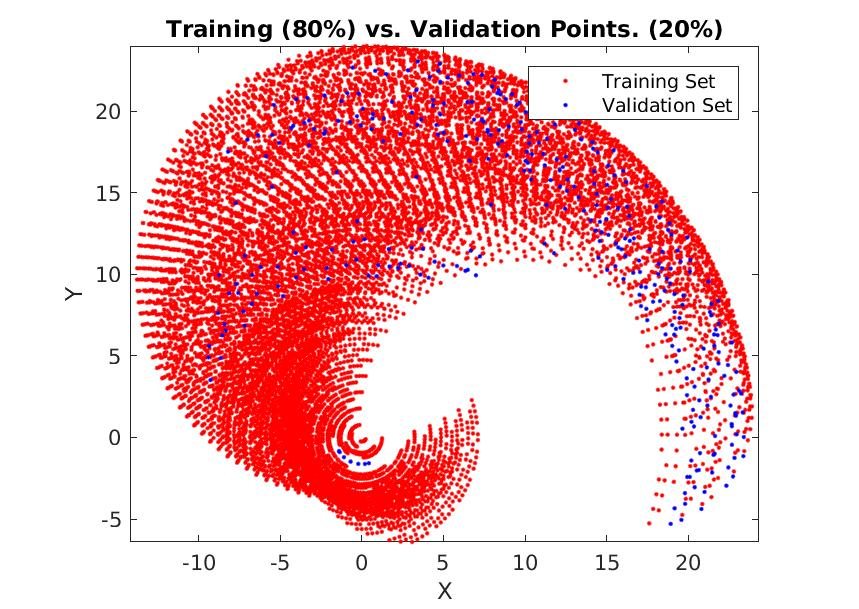
\includegraphics[width=1\textwidth]{trnvsval80.jpg}
		\caption{80:20 split.}
		\label{fig::1a}
	\end{subfigure}
	~
	\begin{subfigure}{0.48\textwidth}
		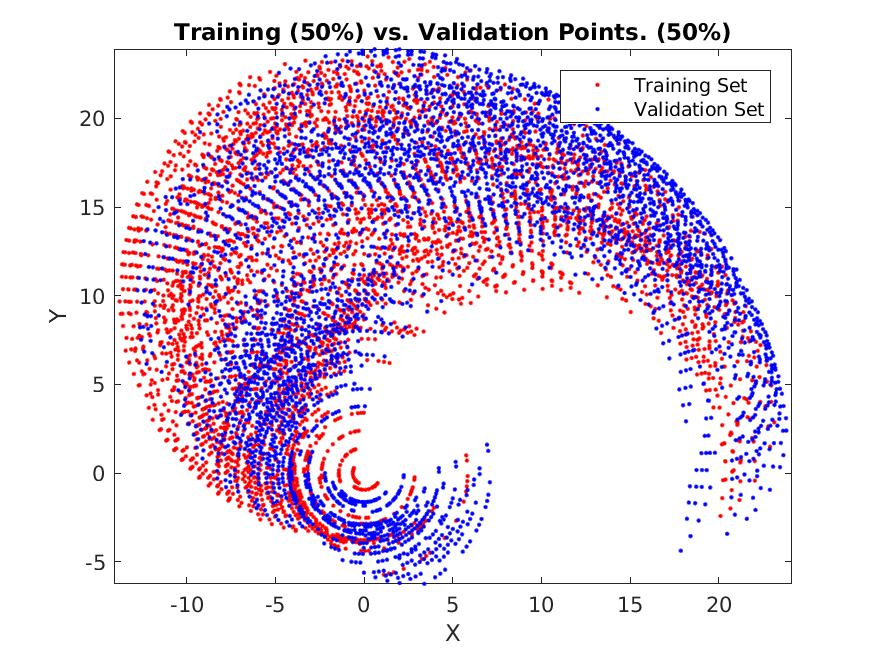
\includegraphics[width=1\textwidth]{trnvsval50.jpg}
		\caption{50:50 split.}
		\label{fig::1b}
	\end{subfigure}	
	\begin{subfigure}{0.48\textwidth}
		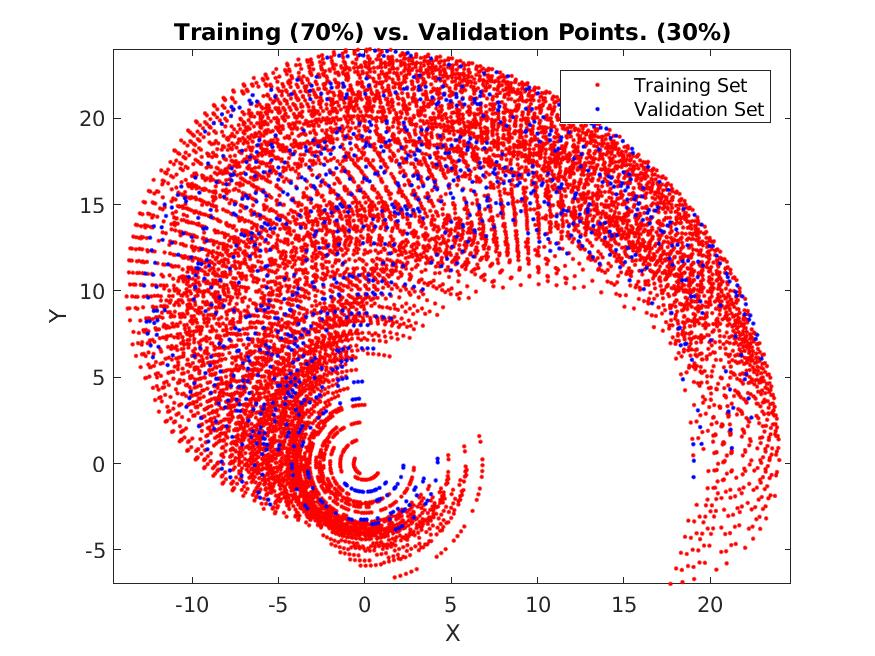
\includegraphics[width=1\textwidth]{trnvsval70.jpg}
		\caption{70:30 split.}
		\label{fig::1c}
	\end{subfigure}	
	\begin{subfigure}{0.48\textwidth}
		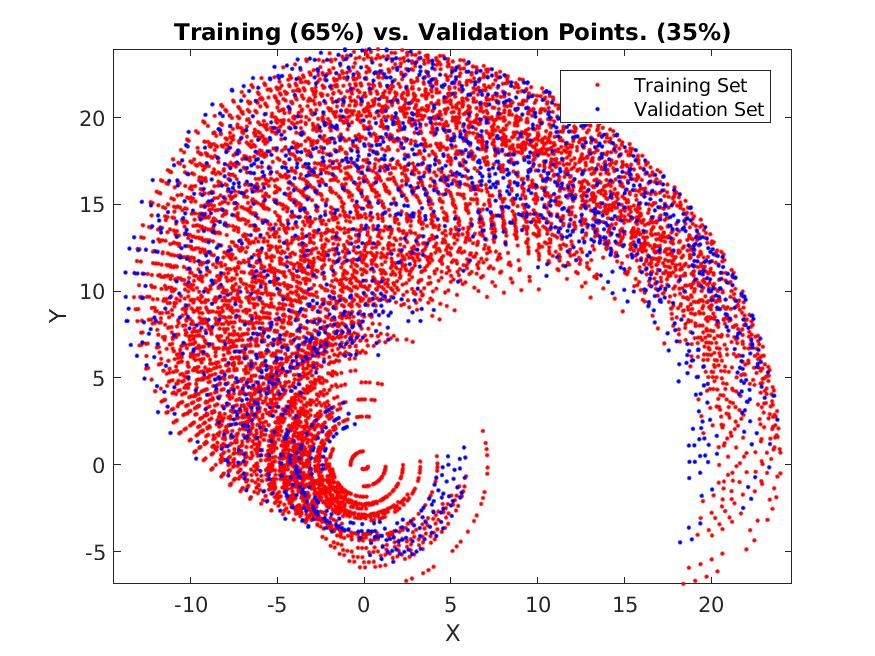
\includegraphics[width=1\textwidth]{trnvsval65.jpg}
		\caption{65:35 split.}
		\label{fig::1d}
	\end{subfigure}	
	\caption{Workspace plots for different training and validation dataset splits.}
	\label{fig::1}
\end{figure}

\newpage
\subsection{ANFIS vs. Neural Network}
\subsubsection{Method}
\subsubsection{Results and Discussion}

\newpage
\subsection{Singularity Considerations}
\subsubsection{Method}
\subsubsection{Results and Discussion}

\newpage
\subsection{Search Algorithm for Parameters}
\subsubsection{Method}
\subsubsection{Results and Discussion}

\newpage
\section*{Appendix}

\begin{lstlisting}[language=MATLAB]
\end{lstlisting}

\newpage
\bibliographystyle{plain}
\bibliography{/home/aegeus/Desktop/MSc/Papers/library}


\end{document}
